
	\section{ACM/ICPC World Finals 2011}
		\subsection{ACM/ICPC World Finals 2011 A To Add or to Multiply}
			\subsubsection{题目大意}
				给定 $a,b,p,q,r,s$。一个程序定义为 对输入的数进行一系列加 $a$ 和乘 $b$ 的操作,并返回最终结果 的操作序列。设计一个程序 $f$,使得任意输入 $x \in [p,q]$,保证输出 $f(x) \in [r,s]$。请先最小化程序的操作总数,再最小化其字典序,并将最优的程序输出。加法 $<$ 乘法。
					
				$a,b,p,q,r,s$ 均为正整数,且 $   \le\num{1e9} $。$p\le q, r\le s$。
			\subsubsection{算法讨论}
				注意到乘法操作是有限的。若 $b=1$,那么乘法操作没有作用,无需执行;否则,设进行了 $multi$ 次乘法操作,那么最大的输出至少为 $q b^{multi}$。要保证输出 $f(x) \le s$ ,就要保证
				\begin{align}
					q b^{multi} &\le s
					\intertext{即}
						 multi& \le \log_b ( s/q)
				\end{align}
				本题中此上限为  $29 (s = \num{1e9},q=1,b=2)$。所以,不妨先枚举 $multi$ 的值。
						
				随后需要考虑加法的操作。设在第 $i$ 次乘法和第 $(i+1)$ 次乘法操作间插入了 $h_{multi-i}$ 次加法操作,特殊地,$h_{multi},h_0$ 分别表示一开始和最后执行的加法操作数。那么对于输入  $x \in [p,q]$,输出
				\begin{align}
					f(x) \in \left[ p b^{multi} + a\Delta ,q b^{multi} + a\Delta \right ] \subset [r,s]
				\end{align}
				其中 $\Delta = \sum_{i=0}^{multi} h_ib^i$。整理得
				\begin{align}
						\frac{r-p b^{multi}}{a} \le \Delta \le \frac{s - q b^{multi} }{a} \label{jiachengzhengli}
				\end{align}
				将 \eqref{jiachengzhengli} 简记为  $u \le \Delta \le v$。那么问题转化为,求一组 $h$,在满足 \eqref{jiachengzhengli} 的情况下,先最小化总和,再最大化 $h$ 的字典序。此问题可以由一个贪心算法解决。从 $h_{multi}$ 起,逐渐增加其值。如果 $\Delta \ge u$,那么构造算法结束;如果将当前的 $h_{\cdot}$ 再增加一会导致  $\Delta > v$,则停止当前位的枚举,转更低位置的 $h_{\cdot}$。这个贪心算法的正确性的证明可以参考进位制。
				\begin{pf}
					设某个 $h$ 的较高位 $h_i$ 本来可以增加一,即 $\sum_{j=0}^{(i-1)} h_jb^j \ge b^i$,那么必然 $ \exists j<i, h_j\ge b$(否则 $\sum_{j=0}^{(i-1)} h_jb^j \le \sum_{j=0}^{(i-1)} (b-1)b^j = b^i -1 < b^i$ 矛盾。)将 $h_j$ 减少 $b$,$h_{(j+1)}$ 增加 $1$。重复以上过程有限次,即可使得 $h_i$ 增加,且 $h$ 的总和在不断减少,新序列会不断地变优,$\Delta$ 也未发生变化。重复寻找新的 $i$ 并且反复更新即可使得任意序列变化为贪心算法给出的解。\qed
				\end{pf}
				显然,上述算法给出的也就是字典序最大的解。
					
				最后,选择各个 $multi$ 值中,答案最优的解输出。 
			\subsubsection{时空复杂度}
				时间复杂度 $\mathcal{O}\left(\log_b^2 ( s/q)\right)$。
					
				空间复杂度 $\mathcal{O}\left(\log_b ( s/q)\right)$。
		\newpage
		\subsection{ACM/ICPC World Finals 2011 B Affine Mess}
			\subsubsection{题目大意}
				给定三个整点构成的点集 $x$。先进行一次未知的旋转变换,再进行未知的伸缩变换和未知的平移变换。已知伸缩变换的系数为非零整数,平移变换的量为整数。旋转变换会使得原来的 $x$ 轴移动到正方形
				$
						D : -10\le x,y\le 10
				$
				的边界的整点上,并把变换后的坐标四舍五入取整。已知 $x$ 经过上述复合变换 $f$ 后变为集合 $y$。试问是否存在 $f$ 以及 $f$ 是否本质相同。本质相同指变换 $ f(\mathbf{x}) = A \mathbf{x} + \mathbf{b}$ 的 $A,\mathbf{b}$ 是唯一的。粗体表示向量。
					
				$x$ 中的坐标的绝对值 $\le 500$,均为整数。
			\subsubsection{算法讨论}
				旋转变换只有 40 种($D$ 边界上,极角 $\in [0,\pi)$ 的整点数)。集合 $x$ 与集合 $y$ 的双射情况只有 $3! = 6$ 种。可先枚举。
				
				随后 $x$ 变换为 $x_0 = \left\{\left(x_1,y_1\right),\left(x_2,y_2\right),\left(x_3,y_3\right)\right\}$。
				设  $y = \left\{\left(X_1,Y_1\right),\left(X_2,Y_2\right),\left(X_3,Y_3\right)\right\}$。问题则变为,是否存在且是否唯一地存在整数 
				$k_x,b_x,k_y,b_y(k_x \ne 0, k_y \ne 0)$ 满足
				\begin{align}
					\begin{cases}
						X_1 = k_x x_1 + b_x\\
						X_2 = k_x x_2 + b_x\\
						X_3 = k_x x_3 + b_x
					\end{cases}
					\text{ 且 } \,\,\,\,\,\,
					\begin{cases}
						Y_1 = k_y y_1 + b_y\\
						Y_2 = k_y y_2 + b_y\\
						Y_3 = k_y y_3 + b_y
					\end{cases}
				\end{align}
				 两个方程组形式类似。以第一个方程组为例,可视为是否存在直线 $y=kx+b, k\ne 0, k\in \mathbb{Z},b \in \mathbb{Z}$ 经过 $(x_1,X_1), (x_2,X_2), (x_3,X_3)$。如果任意两点横坐标相同,纵坐标不同,那么无解($k$ 取无穷大)。如果三点重合,那么整系数整截距的一次函数有无穷多个,返回多解。如果只有两点重合,那么仅能确定一条直线。判断直线的斜率和截距是否为整数,再返回有唯一解或无解。若三点均不重合,那么先判断其是否共线,再判断斜率和截距是否为整数,最后返回唯一解或无解。对第二个方程组也进行相同的操作并合并当前的答案,再累计入总答案之中。
			\subsubsection{时空复杂度}
				时间复杂度 $\mathcal{O}\left(1\right)$。
					
				空间复杂度 $\mathcal{O}\left(1\right)$。
		\newpage
		\subsection{ACM/ICPC World Finals 2011 C Ancient Messages}
			\subsubsection{题目大意}
				给定一个黑白位图,仅包含图
				\ref{11c} 中的符号。各个符号可能会经过拓扑等价处理。请分析各个符号在图中出现的次数。
				\begin{figure}[!htb]
 					\centering
					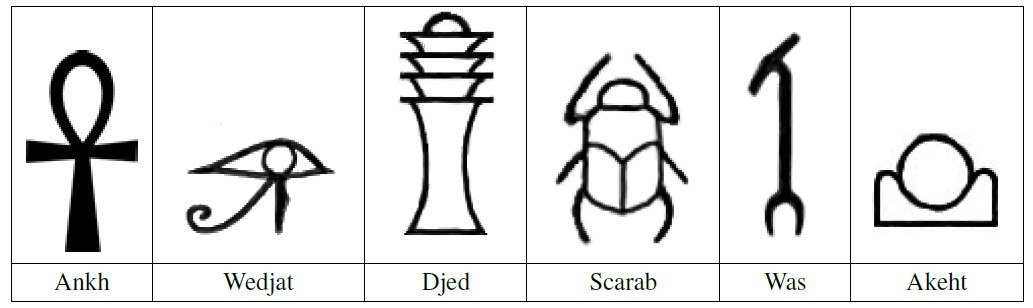
\includegraphics[width=0.8 \textwidth]{6.jpg}
					\caption{位图可能含有的符号}\label{11c}
				
				\end{figure}
				
				位图大小 $N \times M$。$N,M \le 200$。
			\subsubsection{算法讨论}
				经过拓扑等价变换后,图形所含的“空洞”数不会发生变化。恰好,图 \ref{11c} 中的符号的“空洞”数各不相同,可作为辨别它们的依据。
				
				使用 DFS/BFS 算法求出各个极大连通子块所包含的“空洞”数,并与图 \ref{11c} 中个符号的“空洞”数比对,识别之。
			\subsubsection{时空复杂度}
				时间复杂度 $\mathcal{O}\left(NM\right)$。
					
				空间复杂度 $\mathcal{O}\left(NM\right)$。
		\newpage
		\subsection{ACM/ICPC World Finals 2011 E Coffee Central}
			\subsubsection{题目大意}
				矩形 $R: 1\le x \le N, 1 \le y \le M$ 中有若干整点 $(x_i,y_i)$。给定整数 $B$,请另外求一个 $R$ 中的整点 $(x_0,y_0)$,使得原来的整点中满足
				\begin{align}	
					\left|x_i-x_0\right|+\left|y_i-y_0\right| \le B \label{11econstraint}
				\end{align}
				的数量尽可能多。若有多解,先最小化 $y$,再最小化 $x$。 
				
				$N,M \le \num{1000}$。多组测试。一组测试内整点集合是不变的,但有多个待询问的 $B$ 值。
			\subsubsection{算法讨论}
				定义旋转变换 $(x,y) \mapsto (x+y,x-y)$。在此变换下,\eqref{11econstraint} 变为正方形 
				\begin{align}	
					\left\{
						\begin{aligned}
						\left|x_i-x_0\right| & \le B \\
						\left|y_i-y_0\right|& \le B
						\end{aligned}
					\right.
				\end{align}
				那么该正方形内的点数,可以用二维前缀和求出。设 $S[i][j] = \sum_{p\le i \atop q \le j} [(p,q) \text{ 在变换后的点集中}]$。
				\begin{align}	
					S[i][j]=[(i,j) \text{ 在变换后的点集中}] +S[i-1][j]+S[i][j-1]-S[i-1][j-1]
				\end{align}
				对于正方形 $(x_1,y_1) - (x_2,y_2)$,正方形内的点数
				\begin{align}	
					Ans = S[x_2][y_2]-S[x_2][y_1-1]-S[x_1-1][y_2]+S[x_1-1][y_1-1]
				\end{align}
				枚举要选择的点并 $\mathcal{O}(1) $ 计算点数。
			\subsubsection{时空复杂度}
				时间复杂度 $\mathcal{O}\left(NM\right)$。
					
				空间复杂度 $\mathcal{O}\left(NM\right)$。
		\newpage
		\subsection{ACM/ICPC World Finals 2011 F Machine Works}
			\subsubsection{题目大意}
				有 $N$ 个物品。第 $i$ 个物品只能在第 $D_i$ 天买到,价格 $P_i$,回收价 $R_i, P_i > R_i$,回收时间任意,但必须严格在第 $D_i$ 之后。每天只能持有一件物品,
				且从买入第二天起,持有第 $i$ 件物品将会带来 $G_i$ 的收入。过程持续 $D, D_i \le D$ 天,第 $(D+1)$ 天,持有物会被强制回收。
				初期成本 $C$。 求整个过程的最大收益加本金。
			
				$N \le \num{1e5}$。
			\subsubsection{算法讨论}
				构造两个虚拟物品 $i=0,N+1$,分别在第 $0,(D+1)$ 天上市,价格均满足 $P_i,R_i,G_i = 0$。然后,对物品按 $D_i$ 排序。
				
				设 $F[i]$ 表示目前持有物品 $i$ 的收益,则
				\begin{align}
					F[i] &= \max_{j<i} F[j]+(D_i-D_j) \cdot G_j-P_i+R_i
					\intertext{由于最优方案的收益一定随时间单调不降,故只需检测当前本金加利润是否超过 $P_i$,即
					\begin{align}
						F[i]+C-R_i+P_i < P_i
					\end{align}
					若满足上式,则将 $F[i]$ 重置为 $+\infty$。边界
					}
					F[0] &=0
					\intertext{答案}
						Ans &=F[N+1]+C
				\end{align}		
					
				暴力实现耗时 $\mathcal{O}\left(N ^2\right)$。使用斜率优化可降为 $\mathcal{O}\left(N\log N\right)$。
				本题中,斜率单调,但横坐标不单调,故需用数据结构维护凸壳。可以根据斜率删掉之后无用的点,故不需二分最优点。
			\subsubsection{时空复杂度} 
				时间复杂度 $\mathcal{O}\left(N \log N\right)$。
					
				空间复杂度 $\mathcal{O}\left(N\right)$。
		\newpage
		\subsection{ACM/ICPC World Finals 2011 H Mining Your Own Business}
			\subsubsection{题目大意}
				给定无向图 $G=(V,E)$。求点集 $V^\prime \subset V$,使得删去 $G$ 任意一点后,各极大连通分量均存在至少一个点在 $V^\prime$ 中。求最小的 $|V^\prime|$ 以及达到此最小值的方案。
				
				$N = |V| \le \num{5e4}$。
			\subsubsection{算法讨论}
				显然只有割点被删去之后,图的连通性才会发生变化。不妨先求出各个割点。
				
				在原图中删去所有割点,并分别考虑形成的极大连通块。如果该连通块仅与一个割点连接,那么必须在该连通块中选择任意一个结点放入  $V^\prime$  中,方案数为连通块大小。原因是如果此割点被删除,就会违背题目条件。
				
				如果连通块与多个割点连接,那么无需将任何结点放入  $V^\prime$  中,方案数为 1。因为任意割点被断掉后,仍然可通过其他的割点走到属于 $V^\prime$ 的结点。
					
				如果连通块无任何割点连接,那么需放置至少两个结点到 $V^\prime$  中,方案数 $\binom{\text{连通块大小}}{2}$。原因是断掉任意节点虽然无连通性的变化,但至少还要保证一个没有被删掉的结点还在 $V^\prime$ 中。
				
				
			\subsubsection{时空复杂度}
				时间复杂度 $\mathcal{O}\left(N\right)$。
					
				空间复杂度 $\mathcal{O}\left(N\right)$。
		\newpage
		
		\subsection{ACM/ICPC World Finals 2011 I Mummy Madness}
				
				\begin{wrapfigure}{r}{0.35 \textwidth}
					\centering
					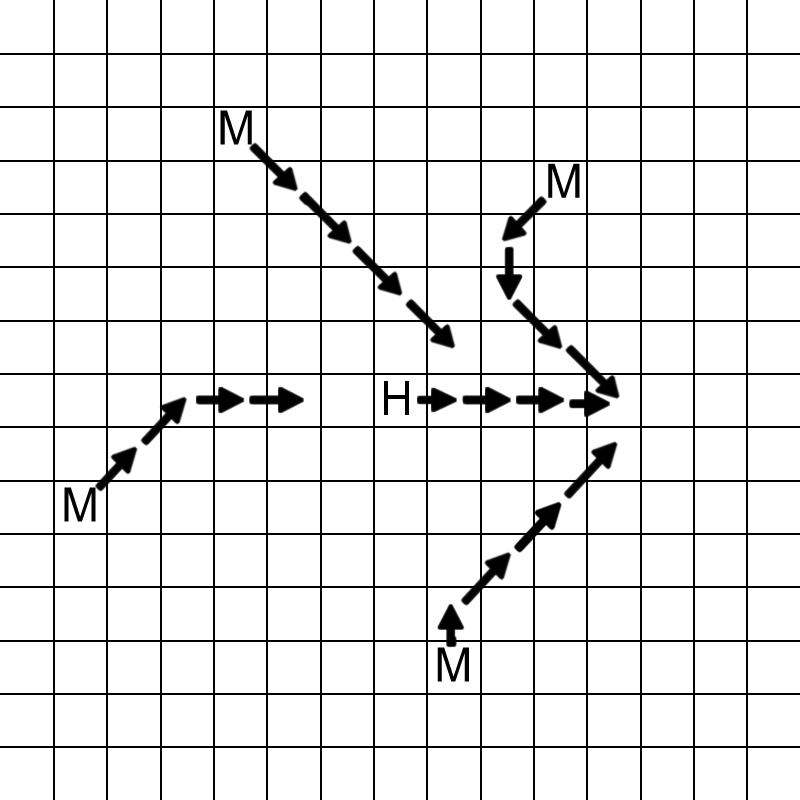
\includegraphics[width=0.3 \textwidth]{5.png}
					\caption{一个可能的局面}
				\end{wrapfigure}
			\subsubsection{题目大意}
				在二维网格中,有一个玩家和 $N$ 个僵尸。玩家每次可以向周围的八个格子移动;随后,\emph{每个}僵尸会\emph{各自}向周围八个格子中,离玩家最近的一个格子移动一步。距离以欧几里德距离计($d = \sqrt{\Delta x^2 + \Delta y^2}$)。一旦僵尸与玩家重合,游戏结束。试问游戏最长能进行多久?
				
				$N \le \num{1e5}$,初始时人和僵尸不重合。
			\subsubsection{算法讨论}
				假定开始时刻 $x = 0$。设 $f(x)$ 表示是否存在一种策略,使得游戏能进行到时刻 $x$。显然 $f(x)$ 关于 $x$ 单调,而答案即使得 $f(x)$ 为真的最大 $x$(可能是 $+ \infty$)。确定答案上界后,不难用二分答案求出答案。
				
				对于特定 $x$,如何求出 $f(x)$ 呢。
				
				记 $R_i$ 表示以第 $i$ 个僵尸为中心,长宽为 $(2 x + 1)$ 且与坐标轴平行的正方形; $R_0$ 表示以人为中心,长宽为 $(2 x + 1)$ 且与坐标轴平行的正方形。
				\begin{theorem}
					直到时刻 $x$,玩家可以躲过所有僵尸当且仅当 $R_0 \setminus (R_1 \cup R_2 \cup \ldots R_N) \ne \varnothing$
				\end{theorem}
				\begin{pf}
					先证充分性。若 $R_0 \setminus (R_1 \cup R_2 \cup \ldots R_N) = A \ne \varnothing$,那么从 $A$ 中任选一个节点 $x$,并\emph{尽早}走向它。
					
					考虑横坐标的投影(纵坐标类似),则玩家需要一路向着 $x$ 行走直到到达 $x$ 后停下。由于
$(R_1 \cup R_2 \cup \ldots R_N)$ 就是所有僵尸在不追玩家的情况下能到达的地方,那么到达 $x$ 后,不管僵尸怎么追,都不会追上主角,故此情况成立。而到达 $x$ 前,对于主角投影点在 $R_i$ 投影区间 中的僵尸 $i$,由于各区间等长,故主角必然向远离 $i$ 的方向运动,在该方向的投影的距离不会变化,故同样追不上主角。综上,必要性成立。
					
					下证必要性。若 $R_0 \setminus (R_1 \cup R_2 \cup \ldots R_N) = \varnothing$,那么不管怎么走,主角都会落入某一个僵尸 $i$ 的 $R_i$ 中。
					
					还是考虑两个方向投影,在主角的投影点与(前文中的)僵尸 $i$ 重合之前,僵尸 $i$ 会一直向着主角的投影方向前进。由于区间等长,如果僵尸 $i$ 的投影从未遇到过主角的投影,那么这个僵尸会走到 $R_i$ 的投影区间中靠近主角的一端;换言之,主角在 $x$ 时不会进入 $R_i$ 的投影区间,与假设矛盾。故总有一刻,其会与主角重合。忽略游戏的停止,假设游戏继续进行,则此僵尸会一直与主角重合。综上,时刻 $x$ 时,僵尸 $i$ 与主角仍会重合,游戏结束,充分性成立。 \qed
				\end{pf}
				根据上述定理,只需用扫描线 + 线段树来确定 $R_0 \setminus (R_1 \cup R_2 \cup \ldots R_N)$ 是否为空即可。具体的,设横坐标为时间轴,纵坐标用线段树维护,那么所有正方形的左边为区间插入事件,右边则为区间删除事件。只需注意是否存在一刻,线段树某个位置上为空。具体的可用打标记的方法实现。有两个标记,一个是此子区间被(完整)覆盖的次数,二是忽略上述的完整覆盖,有多少位置为空。
				
				答案的上限取一个足够大的整数 $U$ 即可。
			\subsubsection{时空复杂度}
				时间复杂度 $\mathcal{O}\left(\log U \cdot(N \log N + N \log U + U)\right)$。使用离散化后,时间复杂度 $\mathcal{O}\left(N \log N\log U\right)$。
					
				空间复杂度 $\mathcal{O}\left(U + N\right)$。
		\newpage
		\subsection{ACM/ICPC World Finals 2011 J Pyramids}
			\subsubsection{题目大意}
				有 $N$ 个木块。搭建一个高度为 $h$ 的\emph{大}金字塔需木块
				\begin{align}
					f(h) & = \sum_{i = 1}^{h} i^2 = (1/6) \cdot  h \cdot (h + 1) \cdot (2 h + 1)
				\intertext{个;搭建一个高度为 $h$ 的\emph{A 型小}金字塔需木块}
					g(h) & = \sum_{i = 1}^{h} {(2i - 1)}^2 = (1/3) \cdot h \cdot (2 h-1) \cdot  (2 h+1)
				\intertext{个;搭建一个高度为 $h$ 的\emph{B 型小}金字塔需木块}
					h(h)  &  = \sum_{i = 1}^{h} {(2i)}^2 = (2/3) \cdot  h \cdot (h + 1) \cdot (2 h + 1)
				\end{align}
				个。要求
				\begin{enumerate}
					\item 用上所有的 $N$ 个木块;
					\item 搭尽量少的金字塔,但必须\emph{超过}一个;
					\item 任意两个金字塔尺寸不同;
					\item 任意金字塔的高度 $h$ \emph{至少为} $2$;
					\item 按金字塔的木块数从大到小排序后,此序列的字典序最大。
				\end{enumerate}
				并输出方案。
				
				$1 \le N \le \num{1e6}$。
				
			\subsubsection{算法讨论}
				枚举可知,满足 $h \ge 2$ 且 $f(h), g(h), h(h) \le N \le \num{1e6}$ 的 $f(h), g(h), h(h)$ 不超过 $a = 321$ 个%,且所需木块数量两两不同
				。
				将其视为物品,进一步使用背包算法求各个大小下最少的物品数可知,任意大小  $1 \le N \le \num{1e6}$,只要存在合法摆法,那么总存在不超过 $b = 6$ 个金字塔的摆法。故在背包算法中,在每一个状态里再辅助计入方案情况,按照题面的信息取最优值即可。
			\subsubsection{时空复杂度}
				时间复杂度 $\mathcal{O}\left(a b N\right)$。
				
				空间复杂度 $\mathcal{O}\left(b N\right)$。$a, b$ 意义同前。
		\newpage
		\subsection{ACM/ICPC World Finals 2011 K Trash Removal}
			\subsubsection{题目大意}
				求\emph{简单}多边形的最小直径。最小直径定义为将多边形旋转某一角度后,多边形内点的纵坐标的最大最小值之差。
				
				多边形顶点数 $n \le \num{100}$。
			\subsubsection{算法讨论}
				一种方法是先求其凸包,再旋转卡壳。
				
				另一种方法是直接对其旋转卡壳。枚举一块木板卡住的两点 $A, B$,枚举另一个木板上可能被卡住的点 $C$。
				那么要求
				\begin{align}
					\forall C, \quad \quad \overrightarrow{AB} \times \overrightarrow{AC} \ge 0 \label{K Trash Removal 1}
				\end{align}
				因为若 \eqref{K Trash Removal 1} 不满足,那么木板就将多边形分成了两半。答案即
				\begin{align}
					Ans = \max_C \frac{ \overrightarrow{AB} \times \overrightarrow{AC}}{ \sqrt{ {\overrightarrow{AB}}^2 }} \label{K Trash Removal 2}
				\end{align}
				因为 \eqref{K Trash Removal 2}  是另一个木板应存在的位置。
				此处叉积定义为空间叉积在 $z$ 轴的投影,即
				\begin{align}
					(x_1, y_1) \times(x_2, y_2) = \begin{vmatrix} x_1 & y_1 \\ x_2 & y_2 \\\end{vmatrix}
				\end{align}
				
				有一些常数优化,例如枚举了 $\overrightarrow{AB}$ 就不必再枚举 $\overrightarrow{BA}$,而只需在枚举 $\overrightarrow{AB}$ 时将计算出的值取反等等。
			\subsubsection{时空复杂度}
				先求其凸包,再旋转卡壳:时间复杂度  $\mathcal{O}\left(N\right)$。
				
				直接旋转卡壳:时间复杂度  $\mathcal{O}\left(N^3\right)$。
				
				空间复杂度 $\mathcal{O}\left(N\right)$。
				
				
		\newpage
				